%% packages
\documentclass{article}
\usepackage[a4paper, left=2.0cm, right=2.0cm, top=3.5cm]{geometry}
\usepackage[ngerman]{babel}
\usepackage{graphicx}
\usepackage{multicol}
\usepackage{amssymb}
\usepackage{titlesec}
\usepackage{wrapfig}
\usepackage{blindtext}
\usepackage{lipsum}
\usepackage{caption}
\usepackage{listings}
\usepackage{fancyhdr}
\usepackage{nopageno}
\usepackage{authblk}
\usepackage{amsmath} % tons of math stuff
\usepackage{mathtools} % e.g. alignment within matrix
%\usepackage{bm} % provides shorthand for bold in math mode
\usepackage{dsfont} % \mathds makes double stroke digits
\usepackage{esdiff} % provides \diff
%\usepackage[ISO]{diffcoeff}
\usepackage{xcolor}
\usepackage{csquotes} % e.g. provides \enquote
\usepackage[separate-uncertainty=true]{siunitx} % units
\usepackage{xcolor} % colored text
\usepackage{csvsimple}
\usepackage{subcaption}
\usepackage{physics}
\usepackage{hyperref}
\usepackage{nameref}
\hypersetup{colorlinks=true, linkcolor=black, pdfhighlight={/N}}
\usepackage{tcolorbox}
\usepackage{amsthm}




%\fancyhf[]{}

%% custom stuff
% own units
\DeclareSIUnit \VSS {\ensuremath{V_\mathrm{SS}}}
\DeclareSIUnit \VS {\ensuremath{V_\mathrm{S}}}
\DeclareSIUnit \Veff {\ensuremath{V_\mathrm{eff}}}
\DeclareSIUnit \Vpp {\ensuremath{V_\mathrm{pp}}}
\DeclareSIUnit \Vp {\ensuremath{V_\mathrm{p}}}
\DeclareSIUnit \VRMS {\ensuremath{V_\mathrm{RMS}}}
\DeclareSIUnit \ASS {\ensuremath{A_\mathrm{SS}}}
\DeclareSIUnit \AS {\ensuremath{A_\mathrm{S}}}
\DeclareSIUnit \Aeff {\ensuremath{A_\mathrm{eff}}}
\DeclareSIUnit \App {\ensuremath{A_\mathrm{pp}}}
\DeclareSIUnit \Ap {\ensuremath{A_\mathrm{p}}}
\DeclareSIUnit \ARMS {\ensuremath{A_\mathrm{RMS}}}

% change subsection numbering to capital letters
\newcommand{\subsectionAlph}{ \renewcommand{\thesubsection}{\arabic{section}.\Alph{subsection}} }
% change subsection numbering to lowercase letters
\newcommand{\subsectionalph}{ \renewcommand{\thesubsection}{\arabic{section}.\alph{subsection}} }
% change subsubsection numbering to lowercase letters
\newcommand{\subsubsectionalph}{ \renewcommand{\thesubsubsection}{\arabic{section}.\arabic{subsection}.\alph{subsubsection}} }
% own fig. that works with multicols
\newenvironment{Figure}
  {\par\medskip\noindent\minipage{\linewidth}}
  {\endminipage\par\medskip}
\newcommand*{\inputPath}{./plot} % prepend this command to the argument of all input commands
\graphicspath{ {./images/}{./figure/}{../plot/} }
% own enviroment for definitions
\newenvironment{definition}[1]
{\begin{quote} \noindent \textbf{\textit{#1\ifx&#1& \else : \fi}} \itshape}
{\end{quote}}


% own commands
% \newcommand{\rarr}{$\to\,$} %A$\,\to\,$B
\newcommand{\defc}{black}
\newcommand{\colorT}[2][blue]{\color{#1}{#2}\color{\defc}}
\newcommand{\redq}{\color{red}(?)\color{\defc}}
\newcommand{\question}[1]{\colorT[purple]{\textbf{(#1)}}}
\newcommand{\todo}[1]{\colorT[red]{\textbf{(#1)}}}
\newcommand{\mr}{\mathrm}

%% preparation
\begin{titlepage}
    \title{Praktikum Atome, Moleküle, kondensierte Materie \\ Versuch 402}
    \author[1]{Carlos Pascua\thanks{s87cpasc@uni-bonn.de}}
    \author[1]{Michael Vogt\thanks{s65mvogt@uni-bonn.de}}
    \affil[1]{Uni Bonn}
    %\date{\today}
\end{titlepage}


%% document
\begin{document}

\pagenumbering{gobble}
\maketitle
\tableofcontents
\newpage
\pagenumbering{arabic}

\pagestyle{fancy}
\fancyhead[R]{\thepage}
\fancyhead[L]{\leftmark}

\section*{Einleitung}


\section{Teil l: Bestimmung des Planckschen Wirkungsquantum}
  \subsection{Theorie}

    \subsubsection{Photoeffekt}

    \subsubsection{Gegenfeldmethode}

    \subsubsection{Photozelle}
\subsection{Aufbau und Durchführung}

\subsection{Beobachtungen und Auswertung}

\subsection{Diskussion}

\clearpage
\section{Fazit}


\clearpage
\section{Anhang}

% Corrected Table for Messung 1a 365 nm data
\begin{table*}[h!]
  \centering
  \begin{tabular}{|c|c|}
      \hline
      $U_0$ [mV] & $I$ [pA] \\
      \hline
      0.5   & 97.5 \\
      219.9 & 66.1 \\
      425   & 49.3 \\
      599   & 36.8 \\
      798   & 24.0 \\
      1009  & 16.0 \\
      1201  & 7.5  \\
      1414  & 3.0  \\
      1606  & 0.7  \\
      1805  & 0.4  \\
      2092  & 0.3  \\
      2394  & 0.2  \\
      2781  & 0.1  \\
      \hline
  \end{tabular}
  \caption{Messung 1a bei 365 nm}
  \label{tab:messung1a}
\end{table*}

% Corrected Table for Messung 1b 365 nm data
\begin{table*}[h!]
  \centering
  \begin{tabular}{|c|c|}
      \hline
      $U_0$ [V] & $I$ [pA] \\
      \hline
      0.001  & 104.5 \\
      0.241  & 75    \\
      0.523  & 49    \\
      0.749  & 29    \\
      1.011  & 14.6  \\
      1.276  & 7.2   \\
      1.510  & 2.9   \\
      1.761  & 1.9   \\
      1.845  & 1.8   \\
      2.085  & 1.6   \\
      2.388  & 1.6   \\
      2.781  & 1.5   \\
      \hline
  \end{tabular}
  \caption{Messung 1b bei 365 nm}
  \label{tab:messung1b}
\end{table*}

% Corrected Table for Messung 2a 405 nm data
\begin{table*}[h!]
  \centering
  \begin{tabular}{|c|c|}
      \hline
      $U_0$ [V] & $I$ [pA] \\
      \hline
      0.005  & 73.9 \\
      0.211  & 54.3 \\
      0.401  & 30.7 \\
      0.614  & 20.6 \\
      0.804  & 11.3 \\
      1.007  & 4.7  \\
      1.201  & 2.5  \\
      1.405  & 1.6  \\
      1.612  & 1.4  \\
      1.801  & 1.4  \\
      2.024  & 1.3  \\
      2.304  & 1.3  \\
      2.781  & 1.4  \\
      \hline
  \end{tabular}
  \caption{Messung 2a bei 405 nm}
  \label{tab:messung365}
\end{table*}

% Corrected Table for Messung 2b 405 nm data
\begin{table*}[h!]
  \centering
  \begin{tabular}{|c|c|}
      \hline
      $U_0$ [V] & $I$ [pA] \\
      \hline
      0.007  & 69.8 \\
      0.212  & 53.8 \\
      0.388  & 38.0 \\
      0.620  & 19.2 \\
      0.794  & 10.9 \\
      1.005  & 5.2  \\
      1.197  & 2.6  \\
      1.403  & 1.8  \\
      1.607  & 1.7  \\
      1.804  & 1.7  \\
      2.014  & 1.5  \\
      2.298  & 1.8  \\
      2.782  & 1.7  \\
      \hline
  \end{tabular}
  \caption{Messung 2b bei 405 nm}
  \label{tab:messung405}
\end{table*}

% Table for Messung 3a 435 nm data
\begin{table*}[h!]
  \centering
  \begin{tabular}{|c|c|}
      \hline
      $U_0$ [V] & $I$ [pA] \\
      \hline
      0.007 & 273.1 \\
      0.201 & 174.2 \\
      0.417 & 102.8 \\
      0.612 & 54.5  \\
      0.795 & 20.8  \\
      1.005 & 2.8   \\
      1.209 & 0.7   \\
      1.408 & 0.6   \\
      1.607 & 0.1   \\
      1.812 & 0.0   \\
      2.017 & 0.4   \\
      2.311 & 0.0   \\
      2.782 & 0.0   \\
      \hline
  \end{tabular}
  \caption{Messung 3a bei 435 nm}
  \label{tab:messung3a}
\end{table*}

% Table for Messung 3b 435 nm data (Messung am nächsten Tag)
\begin{table*}[h!]
  \centering
  \begin{tabular}{|c|c|}
      \hline
      $U_0$ [V] & $I$ [pA] \\
      \hline
      0.005 & 237.3 \\
      0.214 & 187.6 \\
      0.415 & 110.5 \\
      0.596 & 59.3  \\
      0.802 & 21.0  \\
      0.997 & 4.8   \\
      1.210 & 1.0   \\
      1.386 & 0.5   \\
      1.608 & 0.4   \\
      1.803 & 0.3   \\
      2.026 & 0.3   \\
      2.296 & 0.2   \\
      2.781 & 0.1   \\
      \hline
  \end{tabular}
  \caption{Messung 3b bei 435 nm (Messung am nächsten Tag)}
  \label{tab:messung3b}
\end{table*}
% Table for Messung 4a 546 nm data
\begin{table*}[h!]
  \centering
  \begin{tabular}{|c|c|}
      \hline
      $U_0$ [V] & $I$ [pA] \\
      \hline
      0.005 & 306.5 \\
      0.226 & 117.3 \\
      0.406 & 28.7  \\
      0.596 & 5.1   \\
      0.803 & 4.3   \\
      1.007 & 4.3   \\
      1.208 & 4.4   \\
      1.413 & 4.4   \\
      1.602 & 4.5   \\
      1.803 & 4.4   \\
      2.022 & 4.4   \\
      2.307 & 4.3   \\
      2.781 & 4.3   \\
      \hline
  \end{tabular}
  \caption{Messung 4a bei 546 nm}
  \label{tab:messung4a}
\end{table*}

% Table for Messung 4b 546 nm data
\begin{table*}[h!]
  \centering
  \begin{tabular}{|c|c|}
      \hline
      $U_0$ [V] & $I$ [pA] \\
      \hline
      0.006 & 296.2 \\
      0.203 & 126.4 \\
      0.408 & 27.2  \\
      0.620 & 4.8   \\
      0.792 & 4.1   \\
      1.001 & 4.0   \\
      1.203 & 3.9   \\
      1.408 & 3.9   \\
      1.593 & 4.0   \\
      1.791 & 4.0   \\
      2.020 & 4.0   \\
      2.307 & 4.1   \\
      2.781 & 3.9   \\
      \hline
  \end{tabular}
  \caption{Messung 4b bei 546 nm}
  \label{tab:messung4b}
\end{table*}
% Table for Messung 5a 578 nm data
\begin{table*}[h!]
  \centering
  \begin{tabular}{|c|c|}
      \hline
      $U_0$ [V] & $I$ [pA] \\
      \hline
      0.006 & 133.1 \\
      0.205 & 39.4  \\
      0.405 & 6.6   \\
      0.606 & 4.5   \\
      0.809 & 4.3   \\
      1.006 & 4.2   \\
      1.208 & 4.2   \\
      1.411 & 4.3   \\
      1.615 & 4.5   \\
      1.791 & 4.5   \\
      2.025 & 4.5   \\
      2.318 & 4.5   \\
      2.781 & 4.4   \\
      \hline
  \end{tabular}
  \caption{Messung 5a bei 578 nm}
  \label{tab:messung5a}
\end{table*}

% Table for Messung 5b 578 nm data
\begin{table*}[h!]
  \centering
  \begin{tabular}{|c|c|}
      \hline
      $U_0$ [V] & $I$ [pA] \\
      \hline
      0.006 & 120.8 \\
      0.198 & 32.9  \\
      0.401 & 6.2   \\
      0.614 & 4.4   \\
      0.807 & 4.4   \\
      1.008 & 4.4   \\
      1.218 & 4.4   \\
      1.400 & 4.4   \\
      1.594 & 4.3   \\
      1.811 & 4.3   \\
      2.002 & 4.3   \\
      2.309 & 4.3   \\
      2.782 & 4.4   \\
      \hline
  \end{tabular}
  \caption{Messung 5b bei 578 nm}
  \label{tab:messung5b}
\end{table*}

\begin{figure}[h!]
  \centering
  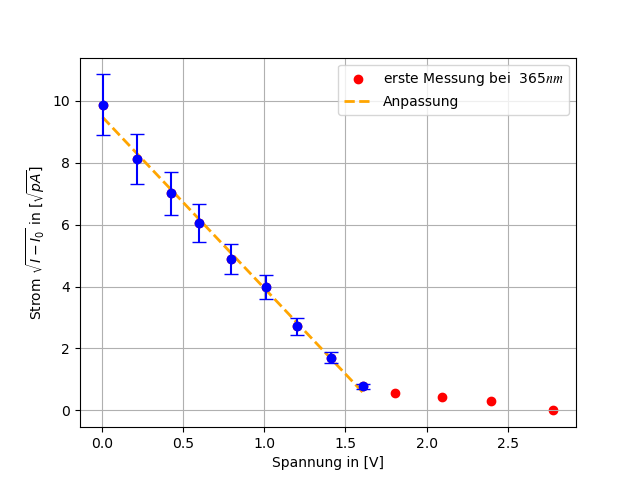
\includegraphics[width=.8\linewidth]{402_365nm_a.png}

  \caption{}
  \label{fig:wellenlaenge_365nm_a}
\end{figure}

\clearpage
\begin{thebibliography}{9}

\bibitem{Anleitung}
\textit{Physikalisches Praktikum Teil IV -- Versuchsbeschreibungen}, Universität Bonn, 10.10.2024


\end{thebibliography}

\end{document}

